\documentclass[12pt]{beamer}
\usetheme{Boadilla}
\usepackage{booktabs}
\usepackage{multirow}
\usepackage{enumitem}
\usepackage{tikz}

\newcommand{\E}{\mathbb{E}}
\usefonttheme{professionalfonts}
\usepackage{pgfplots}
\pgfplotsset{compat=1.18}
\renewcommand{\arraystretch}{1.25}
\usetikzlibrary{trees}
\title[ECON2843]{Lecture 15}
\subtitle{Part 3 Estimation and Hypothesis Test}
\date{}
\usepackage{amsmath,amssymb,mathtools,wasysym}
\begin{document}
	\begin{frame}
		\titlepage
	\end{frame}
	\begin{frame}
		\vspace{1cm}
		\centering
		{\color{blue}\large Continue our talk on hypothesis test}
	\end{frame}
	
\begin{frame}
	\frametitle{Importance of $p$-values}
	
	\begin{itemize}[label={\color{blue}$\blacktriangleright$}]
		\item How can we use $p$-values to conduct a hypothesis test?
		\item A very small $p$-value means that the observed test statistic was very extreme.
		\item So very small $p$-values should result in the rejection of $H_0$.
	\end{itemize}
	
\end{frame}
\begin{frame}
	\frametitle{Importance of $p$-values}
	
	\begin{itemize}[label={\color{blue}$\blacktriangleright$}]
		\item But how small is small?
		\item We can perform the hypothesis test by comparing the $p$-value to the significance level $\alpha$:
		\begin{itemize}[label={\color{blue}$\blacktriangleright$}]
			\item If the $p$-value is less than $\alpha$, we reject $H_0$.
			\item If the $p$-value is greater than $\alpha$, we fail to reject $H_0$.
		\end{itemize}
		\item Why?
		\item Suppose we test $H_0 : \mu = \mu_0$ vs $H_1 : \mu < \mu_0$ at $\alpha = 0.05$.
	\end{itemize}
	
\end{frame}

\begin{frame}
	\frametitle{Importance of $p$-values}
	
\centering
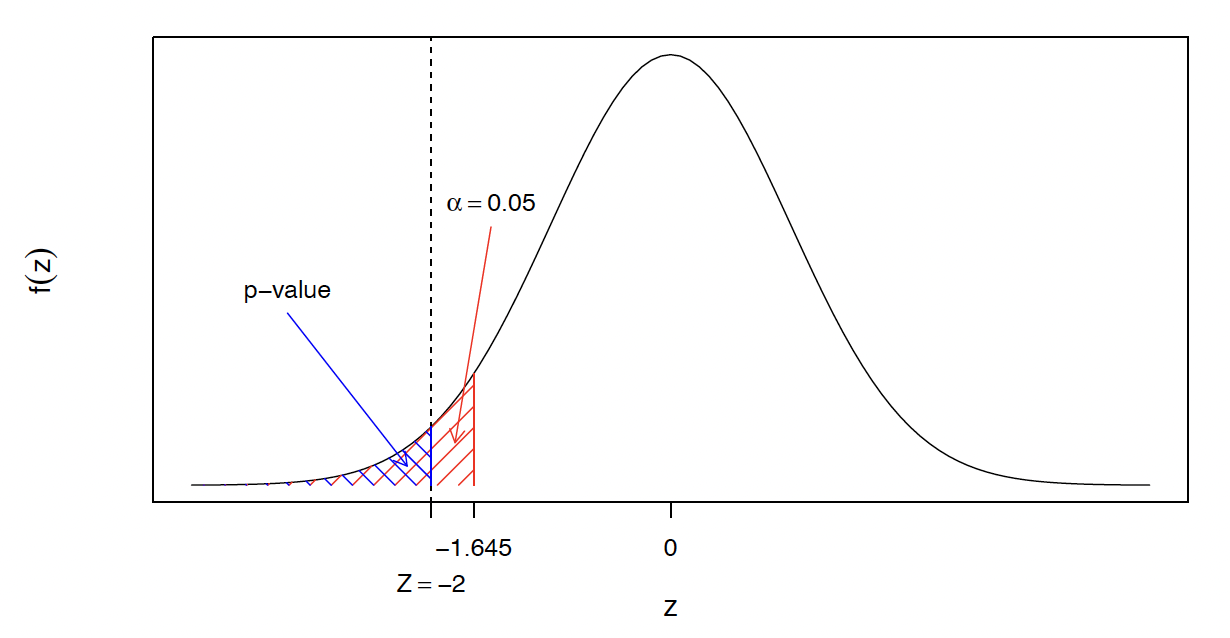
\includegraphics[width=10cm]{importance1.png}	
	
\end{frame}
\begin{frame}
	\frametitle{Importance of $p$-values}
	
	\centering
	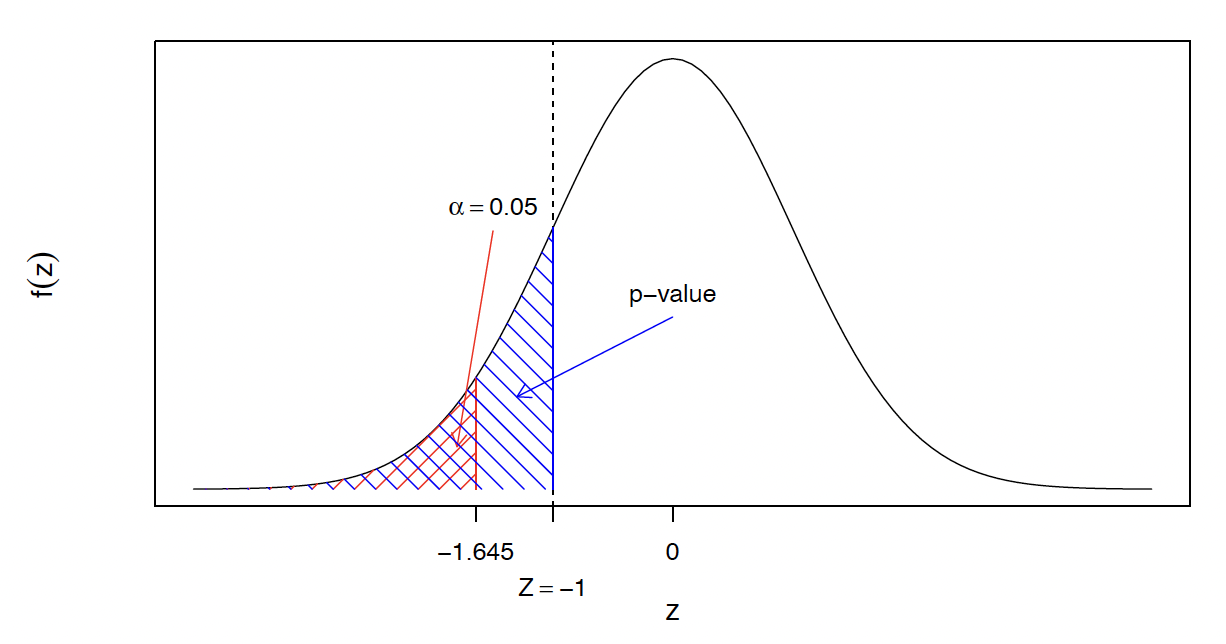
\includegraphics[width=10cm]{importance2.png}	
	
\end{frame}
\end{document}